\chapter{Regulador Linear Quadrático (LQR)}
\label{cap:lqr}

\section{Lei de controle}
Arquivo \code{control/lqr\_controller.cpp}. Sobre o duplo integrador discreto
\eqref{eq:did} (por eixo, mas o código monta a versão 3D bloco-diagonal):
\begin{equation}
  \vect u_k = -K x_k,\qquad
  J=\sum_{k=0}^{\infty} x_k\T Q x_k + u_k\T R u_k,\qquad
  Q=\mathrm{diag}(q_p,q_v),\ R=r .
\end{equation}
$K$ vem da DARE \eqref{eq:dare}, resolvida no construtor por iteração de Riccati até
convergir. Valores do \code{yaml}: $q_p=10$, $q_v=2$, $r=0{,}5$, $\Ts=\SI{0,05}{s}$.

\section{Solução analítica (tempo contínuo)}
Para o duplo integrador contínuo, a equação de Riccati tem solução fechada. Com
$P=\begin{bsmallmatrix}p_1&p_2\\p_2&p_3\end{bsmallmatrix}$:
\begin{equation}
  p_2 = \sqrt{q_p r},\qquad p_3 = \sqrt{r(q_v + 2p_2)},\qquad
  K = \tfrac1r[p_2,\ p_3],
\end{equation}
ou seja,
\begin{equation}
  \boxed{k_p = \sqrt{\frac{q_p}{r}},\qquad
         k_d = \sqrt{\frac{q_v}{r} + 2\sqrt{\frac{q_p}{r}}}}
  \qquad\Longrightarrow\qquad
  \omega_n = \left(\frac{q_p}{r}\right)^{1/4},\quad
  \zeta = \frac{k_d}{2\omega_n}.
  \label{eq:lqr-analitico}
\end{equation}
Com o \code{yaml}: $k_p=4{,}47$, $k_d=3{,}60$, $\omega_n=\SI{2,11}{rad/s}$ e $\zeta=0{,}85$.
A DARE com $\Ts=\SI{0,05}{s}$ dá $K=[4{,}09,\ 3{,}39]$, com polos equivalentes
$s=-1{,}80\pm1{,}11j$ ($\omega_n=2{,}11$, $\zeta=0{,}85$). A discretização reduz os
ganhos em $\approx$\,8\%.

\subsection{Projeto inverso: de especificação para pesos}
Invertendo \eqref{eq:lqr-analitico} com $r=1$ (só as razões importam):
\begin{equation}
  q_p = \omega_n^4,\qquad q_v = 2\omega_n^2\,(2\zeta^2 - 1).
\end{equation}
Consequência: \textbf{com $Q$ diagonal e $q_v\ge0$, o LQR sempre dá $\zeta\ge1/\sqrt2$}.
Para $t_s=\SI{2}{s}$ e $\zeta=0{,}8$: $\omega_n=2{,}5$, $q_p=39$, $q_v=3{,}5$, $r=1$.

\subsection{Regra de Bryson}
Normalize cada variável pelo valor máximo aceitável:
\begin{equation}
  q_i = \frac{1}{x_{i,max}^2},\qquad r = \frac{1}{u_{max}^2}.
\end{equation}
Exemplo: $e_{p,max}=\SI{0,5}{m}$, $e_{v,max}=\SI{1}{m/s}$, $u_{max}=\SI{3}{m/s^2}$ dão
$Q=\mathrm{diag}(4,1)$, $R=0{,}11$, logo $k_p=6{,}0$ e $k_d=4{,}6$. Depois ajuste um
único escalar $\rho$ ($R\leftarrow\rho R$) para trocar desempenho por esforço.

\section{Lugar das raízes simétrico}
Para um sistema SISO com saída ponderada $y = Cx$ ($Q=C\T C$) e $R=\rho$, os polos de
malha fechada do LQR são as raízes estáveis de
\begin{equation}
  1 + \frac{1}{\rho}\,G(-s)\,G(s) = 0,\qquad G(s)=C(sI-A)^{-1}B .
\end{equation}
Esse é o \emph{lugar das raízes simétrico} (Chang--Letov). Ele mostra para onde os polos
vão quando o controle fica ``barato'' ($\rho\to0$: polos rápidos, rumo às assíntotas de
Butterworth) ou ``caro'' ($\rho\to\infty$: polos rumo aos polos estáveis da planta
espelhada, aqui a origem). No MATLAB basta varrer $\rho$ com \code{dlqr}
(\cref{fig:lqr-slgr}).

\begin{figure}[H]
\centering
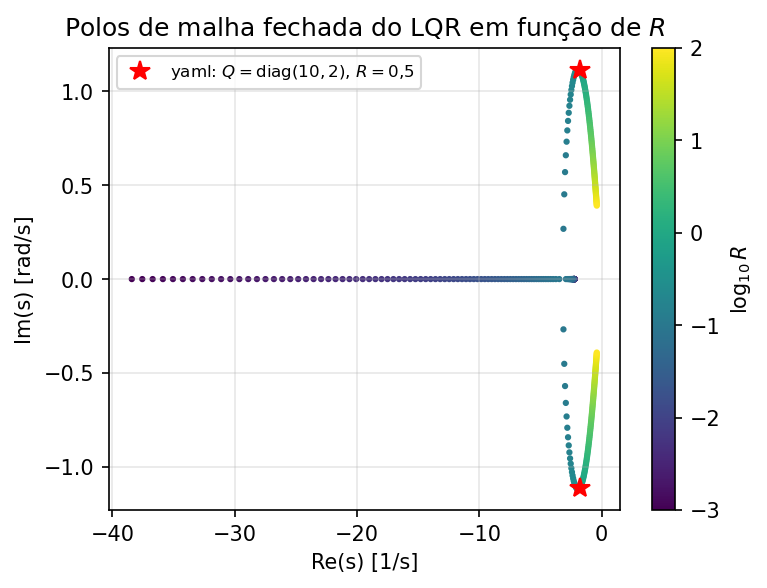
\includegraphics[width=0.62\textwidth]{lgr_lqr_simetrico.png}
\caption{Polos (equivalentes contínuos) do LQR discreto para $Q=\mathrm{diag}(10,2)$ e
$R\in[10^{-3},10^2]$. A estrela marca o \code{yaml}.}
\label{fig:lqr-slgr}
\end{figure}

\section{Robustez e a PX4}
O LQR contínuo com estado completo garante PM $\ge\ang{60}$ e margem de ganho
infinita \emph{na entrada da planta}. Essa garantia \textbf{não vale aqui}, porque:
(i) a PX4 introduz $T_v(s)$ entre o comando e a aceleração real; (ii) há atraso de
medida; (iii) o estado $e_v$ é da referência (\cref{eq:ceq}). A \cref{tab:margens} mostra
PM $=\ang{57}$ sem atraso e \ang{50} com \SI{0,1}{s}. Sempre verifique a margem com o
modelo completo (\code{analise\_margens.m}).

\subsection{LQR com o modelo da PX4 (extensão para o TCC)}
Uma melhoria natural é aumentar o modelo com a dinâmica de aceleração da PX4,
$\dot a = \omega_a(u - a)$, e com a velocidade real:
\begin{equation}
  x = \begin{bmatrix}e_p\\ e_v\\ a\end{bmatrix},\quad
  A_c=\begin{bmatrix}0&1&0\\0&0&1\\0&0&-\omega_a\end{bmatrix},\quad
  B_c=\begin{bmatrix}0\\0\\ \omega_a\end{bmatrix}.
\end{equation}
O ganho resultante $[k_p,k_d,k_a]$ antecipa o atraso da malha interna. Em troca,
exige estimar $a$ (ou usar a aceleração comandada anterior). Com atraso de medida
conhecido, pode-se ainda \emph{prever} o estado para o instante atual,
$\hat x(t) = e^{A\tau}x(t-\tau) + \int_0^\tau e^{A\sigma}Bu\,d\sigma$ (preditor de
Smith em espaço de estados). Ambos estão em \code{projeto\_lqr.m}.

\begin{receita}
\textbf{LQR (\code{matlab/projeto\_lqr.m}).}
\begin{enumerate}
  \item Escolha $Q,R$ por especificação \eqref{eq:lqr-analitico} ou por Bryson.
  \item \code{[K,P,polos] = dlqr(Ad,Bd,Q,R)} com o modelo ZOH de $\Ts=\SI{0,05}{s}$.
        Compare com o C++ (\code{K\_} no construtor).
  \item Varra $\rho$ (LGR simétrico) e escolha o ponto com PM $\ge\ang{45}$ no modelo
        com PX4 + atraso.
  \item Simule em \code{sim\_perseguicao.m}; ajuste $\rho$ pelo índice da comparação.
  \item Copie $q_p,q_v,r$ para \code{lqr.weight\_*} no \code{yaml}.
\end{enumerate}
\end{receita}
